\documentclass[10pt,a4paper,final]{article}
%
\usepackage[utf8x]{inputenc}
\usepackage{ucs}
\usepackage{amsmath}
\usepackage{geometry}
\usepackage{anysize} % Soporte para el comando \marginsize
\usepackage{graphicx}
\usepackage{listings}
\usepackage{amsfonts}
\usepackage{amssymb}
\usepackage[spanish]{babel}
%%%%%%%%%%%%%%%%%%%%%%%%%%%%%%%%%%%%%%%%%%%%%%%%%
%%%%%%%%%%%%%%%%%%%%%%%%%%%%%%%%%%%%%%%%%%%%%%%%%
%%%%%%%%%%%%%%%%%%%%%%%%%%%%%%%%%%%%%%%%%%%%%%%%%
\marginsize{2cm}{2cm}{1.5cm}{1.5cm}
%
\begin{document}
\title{Auditoría Informática de Ing. Química}
\author{Fornal, Esteban, Garbarino, Juan Pablo, Pfarher Christian\\
\textit{Trabajo práctico final de ``Auditoría Informática'', II-FICH-UNL.}}
\markboth{Auditoría Informática: TRABAJO FINAL}{}
\date{\today}
\maketitle
%%%%%%%%%%%%%%%%%%%%%%%%%%%%%%%%%%%%%%%%%%%%%%%%%%%%%%%%%%%%%%%%%%%%%%%%%%%%%%%%
%%%%%%%%%%%%%%%%%%%%%%%%%%%%%%%%%%%%%%%%%%%%%%%%%%%%%%%%%%%%%%%%%%%%%%%%%%%%%%%%
%%%%%%%%%%%%%%%%%%%%%%%%%%%%%%%%%%%%%%%%%%%%%%%%%%%%%%%%%%%%%%%%%%%%%%%%%%%%%%%%
\newpage
\tableofcontents
%%%%%%%%%%%%%%%%%%%%%%%%%%%%%%%%%%%%%%%%%%%%%%%%%%%%%%%%%%%%%%%%%%%%%%%%%%%%%%%%
%%%%%%%%%%%%%%%%%%%%%%%%%%%%%%%%%%%%%%%%%%%%%%%%%%%%%%%%%%%%%%%%%%%%%%%%%%%%%%%%
%%%%%%%%%%%%%%%%%%%%%%%%%%%%%%%%%%%%%%%%%%%%%%%%%%%%%%%%%%%%%%%%%%%%%%%%%%%%%%%%
%\newpage
%\listoffigures % Índice de figuras
%%%%%%%%%%%%%%%%%%%%%%%%%%%%%%%%%%%%%%%%%%%%%%%%%%%%%%%%%%%%%%%%%%%%%%%%%%%%%%%%
%%%%%%%%%%%%%%%%%%%%%%%%%%%%%%%%%%%%%%%%%%%%%%%%%%%%%%%%%%%%%%%%%%%%%%%%%%%%%%%%
%%%%%%%%%%%%%%%%%%%%%%%%%%%%%%%%%%%%%%%%%%%%%%%%%%%%%%%%%%%%%%%%%%%%%%%%%%%%%%%%
\newpage
%%%%%%%%%%%%%%%%%%%%%%%%%%%%%%%%%%%%%%%%%%%%%%%%%%%%%%%%%%%%%%%%%%%%%%%%%%%%%%%%
%%%%%%%%%%%%%%%%%%%%%%%%%%%%%%%%%%%%%%%%%%%%%%%%%%%%%%%%%%%%%%%%%%%%%%%%%%%%%%%%
%%%%%%%%%%%%%%%%%%%%%%%%%%%%%%%%%%%%%%%%%%%%%%%%%%%%%%%%%%%%%%%%%%%%%%%%%%%%%%%%
\section{Presentación}
La Facultad de Ingeniería Química es una institución nacida en 1919 conjuntamente con la Universidad Nacional del Litoral como una casa de altos estudios, con la carrera Ingeniería Química como la principal impulsora de la misma.

\subsection{Misión}
Enmarcada en la Universidad Nacional del Litoral, la Facultad de Ingeniería Química tiene como misión:
\begin{itemize}
\item Transmitir el conocimiento en la búsqueda de su democratización, propendiendo a la elevación del nivel cultural de la comunidad, para que alcance el beneficio de los avances científicos y tecnológicos y las elevadas expresiones de la cultura nacional e internacional.
\item Educar y formar estudiantes y profesionales competentes, críticos y comprometidos con su sociedad, con un conocimiento actualizado, integral y dinámico, fruto de una actividad académica e investigativa autónoma, sistemática e innovadora, que les permita desempeñarse idóneamente en las distintas áreas de su profesión, siempre en la búsqueda y realización de un futuro mejor.
\item Impartir un servicio educativo de excelencia para estudiantes tradicionales y no tradicionales, a niveles de pregrado, grado y posgrado, con programas académicos fundamentados en el pensamiento científico y humanístico, que desarrollen el conocimiento, las destrezas y las actitudes requeridas para el empleo técnico y profesional, para el progreso de la educación y para una participación activa en la sociedad.
\item Generar nuevos conocimientos a partir de actividades de investigación científica-tecnológica rigurosas e interdisciplinarias, tendientes a dar soluciones a las problemáticas locales, regionales y nacionales, y donde la investigación pura y aplicada sean complementarias.
\item Interactuar con el medio socio-productivo, transfiriendo todo su potencial académico, científico y tecnológico, a fin de contribuir al desarrollo económico, social y cultural del país.
\item Afianzar los valores de la libertad, la participación y el respeto por la pluralidad como pilares básicos para una verdadera convivencia democrática.
\end{itemize}
%Presentar formalmente la empresa u organizacion donde se realizara el trabajo
%Se deberá presentar la empresa, negocio, entidad, organismo, clarificando sus objetivos, alcances, ámbito de ingerencia de su accionar, etc.
%Se deberá presentar un organigrama general de la misma, para dar a conocer su estructura jerárquica/funcional, quedando en claro la cantidad aproximada de recursos humanos afectados a la misma.
%Facultad de Ingeniería Química – FIQ
%¿Organigrama general de la FIQ – recursos humanos? Te diría que encares con el que está en la URL que me pasaste (http://www.fiq.unl.edu.ar/autoridades/index.htm\# organizacion y http://www.fiq.unl.edu.ar/catedras/index.htm ) y aclará que no fue posible conseguir el organigrama sin una autorización escrita del decano de la Facultad y que no se cuenta en la institución con un organigrama completo del personal.
%CHRISTIAN: Poner la historia vision mision,, toda la bola esa....poner aca...
\subsection{Ubicación y área de influencia}
La Facultad de Ingeniería Química (FIQ) de la Universidad Nacional del Litoral está emplazada en la ciudad de Santa Fe (Departamento La Capital) de la provincia de Santa Fe (Argentina). 

Cuenta con un edificio principal, denominado \emph{Edificio Gollán}, sito en Santiago del Estero 2829 (ver Figura (\ref{plano_edifs}) cuya imagen se puede ver en la Figura (\ref{edif_gollan}) y sobre el cual se realizó la auditoria (un área del mismo), y un Anexo, \emph{Edificio Damianovich}, que se encuentra ubicado en Santiago del Estero 2654 (ver Figura (\ref{plano_edifs}).

\begin{figure}[tbhp]
\centerline{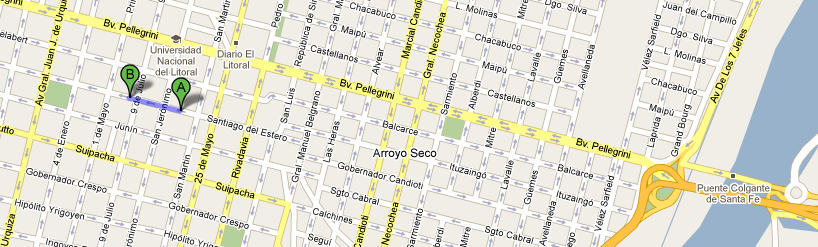
\includegraphics[scale=0.5]{img/plano_edifs}}
\caption{Plano de ubicación de los Edificios Damianovich (A) y Gollán (B)}
\label{plano_edifs}
\end{figure}

\begin{figure}[tbhp]
\centerline{\includegraphics[scale=0.1]{img/edifgollan}}
\caption{Edificio de la Facultad de Ing. química (Edificio Gollán)}
\label{edif_gollan}
\end{figure}

El área de influencia de esta institución, va desde ciudades vecinas hasta Provincias tanto del territorio Nacional como fuera del mismo. Acceden a la misma estudiantes, investigadores y profesores de diferentes ciudades y países del mundo. Aunque cabe aclarar que la mayor población de estudiantes proviene de la provincia de Santa Fe y provincias vecinas.

\subsection{Organigrama de la organización}
no se que vamos a poner.....
%%%%%%%%%%%%%%%%%%%%%%%%%%%%%%%%%%%%%%%%%%%%%%%%%%%%%%%%%%%%%%%%%%%%%%%%%%%%%%%%
%%%%%%%%%%%%%%%%%%%%%%%%%%%%%%%%%%%%%%%%%%%%%%%%%%%%%%%%%%%%%%%%%%%%%%%%%%%%%%%%
%%%%%%%%%%%%%%%%%%%%%%%%%%%%%%%%%%%%%%%%%%%%%%%%%%%%%%%%%%%%%%%%%%%%%%%%%%%%%%%%
\section{Relevamiento}

1- Identificar bien el area donde sta javier y que vamos a auditar.. 
 el bunker de el y laboratorios?, estructura mínima.

2- El área está formada asi:? 

  Sec. Academica 

   |-- piac(7 personas) -- jefe(1:jb) -- resto del personal(6)

   |-- piad (4 personas) 

3- que funcion tiene cada puesto ?

   el jefe:

   el personal:
   
4- programas PIAc, detallar un poco mas que consiste cada programa: para el 
area docente, red de internet..

5)- detallar PIAd, personal no docente y area administrativa..

%----------------------------------------------------------------------
\begin{scriptsize}
A partir de este punto solo se describen aspectos que tienen que ver con la tecnologia
Identificar eo presentar el sector o Area de tecnologia

Orientarse específicamente al área que nos compete, presentando su estructura u organigrama, sus misiones y funciones.
¿Documentación donde pueda obtenerse misión, funciones..? Pagina web? , etc?
¿Organigrama del area informática – recursos humanos?

Existe el "Programa de Informática Académica" (PIAc), dependiente de la Secretaría Académica. Este se encarga de todo lo que es informática para el área docente y red de Internet. Somos siete personas, una de las cuales está afectada al PIAd, para trabajar en el área de desarrollo para Guaraní.

Por otro lado, está el "Programa de Informática Administrativa" (PIAd) , encargada de mantener todo lo que es informática para el personal no docente y áreas administrativas. Son 3 personas, más la que está afectada desde el PIAc.

Los organigramas son "casi" planos: en el caso del PIAc, el cargo otorgado determina la cadena de mandos. O sea, x tener yo el sueldo más alto soy el jefe.  (cero meritocracia :) ), el resto están todos al mismo nivel. Entiendo que el PIAd es similar.
\end{scriptsize}

\subsection{Organigrama del área relevada}
Que funciones y  mision(para que esta.? proveer internet, encargarse de maquinas? admin servidores? cual es la razon de su existencia..) tiene javier como Jefe del piac.

    Organigrama -> funcionalmente de quien depende. (este organigrama esta vinculado con 1.1)
          Dotacion de recursos humanos (cant. para llevar adelante sus objetivos)
%%%%%%%%%%%%%%%%%%%%%%%%%%%%%%%%%%%%%%%%%%%%%%%%%%%%%%%%%%%%%%%%%%%%%%%%%%%%%%%%
%%%%%%%%%%%%%%%%%%%%%%%%%%%%%%%%%%%%%%%%%%%%%%%%%%%%%%%%%%%%%%%%%%%%%%%%%%%%%%%%
%%%%%%%%%%%%%%%%%%%%%%%%%%%%%%%%%%%%%%%%%%%%%%%%%%%%%%%%%%%%%%%%%%%%%%%%%%%%%%%%
\section{Estrategias Informáticas}
\subsection{Estrategias a largo plazo - COMPLETAR}
Unificar los 3 edificios de la FIQ en una sola red de datos.

En los planes a futuro está la migración a linux (o a booteo dual) de las PCs de los gabinetes de docencia.
\subsection{Estrategias a mediano plazo - COMPLETAR}
Completar y trasladar el área de servidores de la FIQ, debido a que está en una oficina de acceso impráctico para trabajar.
\subsection{Estrategias a corto plazo - COMPLETAR}
Mejorar el servicio informático a las cátedras (más un wish que un plan)
Proveer acceso wi-fi a todo el personal docente / no-docente / alumnos de la UNL en la red de la FIQ, sin tantos trámites como se plantean en la red de CETUL (incluído acceso libre pero restringido para quien no pueda autenticarse como perteneciente a la UNL)

\section{Hardware}
1- impresoras, sevidores, hubs, switchs, routers / wifi , tipo y cantidad e maquinas en el bunker y ver si agregamos un laboratorio..
2- caractersiticas basicas del bunker
Presentar los distintos componentes de hardware existentes en la organización. (Cantidad y capacidad).
En el caso de ser muy amplio, informar sólo cantidades.
1- Que tipo de hardware hay en la salita?
2- Como se distribuyen las 300/400 pcs?
Ni idea. Quizás más de 300/400 PCs. Las cátedras son "autárquicas", como todo en la UNL, y el área informática como mucho es un "soporte al que se recurre si se desea". Por lo tanto, no hay un relevamiento formal de equipos.
Puedo darte ideas parciales, si querés...
por ahora no, quiza lo completas luego que arme la estructura en base al link

\section{Software}

\begin{table}
\caption{Software de Base}
\begin{center}\begin{tabular}{ccc}
\hline .NET & Adobe Acrobat Reader\\
\hline Sun Java JRE & PDF Creator\\
\hline Directx & 7zip\\
\hline DocxConverter & Reproductor de Medios VLC\\
\hline Mozilla Firefox & Adobe/Macromedia Flash\\
\hline Openoffice.org & Adobe/Macromedia Shockwave\\
\hline Antivirus AVG & Tight VNC\\
\hline Spybot & \\
\hline
\end{tabular}\end{center}
\label{tablaerrores}
\end{table}

\begin{table}
\caption{Software Administrativo}
\begin{center}\begin{tabular}{ccc}
\hline Office 2003 \\
\hline
\end{tabular}\end{center}
\end{table}

\begin{table}
\caption{Software Gabinetes de Informática}
\begin{center}\begin{tabular}{ccc}
\hline Matlab & Scientific Workplace Pro & Logware\\
\hline Scilab & WinEdt  & Microcal Origin\\
\hline Matemática & Turbo Pascal & TORA\\
\hline R-Project & Arena  & Sybase PowerDesigner\\
\hline WinEdt & Complete FCE & MySQL\\
\hline Tutoriales de Latex & Gabedit & SOFTWARE para LAYOUT\\
\hline Ghostscript & GAMS & Sistema de Informacion\\
\hline Ghostview & Geogebra & Statgraphics\\
\hline Miktex & HYSYS\\
\hline LEd (Std. Ed) & Intellicad\\
\hline
\end{tabular}\end{center}
\end{table}

1- Detallar bien el software que existe en el bunker y el laboratorio o el area que acotemos..
Software (Gral.)
Inventario detallado de los distintos componentes de software de base y software aplicativo, existentes en la organización.
Verificar la existencia de documentación correspondiente a los mismos.

%Mismo que 4. Puedo darte, x ej, el relevamiento del soft instalado en los gabinetes, que dependen de lo que los docentes solicitan para dar clases. Pero eso ni refleja lo que hay en las cátedras ni tampoco representa totalmente lo que se usa en los laboratorios.

El siguiente software es el que está instalado en las PCs de los gabinetes de informática, solicitados por los docentes. 
\emph{agregar tabla de software segun si es base o especifico aca del doc que esta en internet!******************************************************************************}
CHACO: formatear tablas y meterla aca lindas.. sacalas del doc que esta en internet!

Excepto lo que es software libre (FOSS), gratuito o permiso de uso en ambientes académicos, el resto del software utilizado en los gabinetes no cuenta con licencia y está instalado irregularmente. Varios docentes están usando software libre o lo han solicitado al área de informática, pero el personal no está formado en su uso y, por lo tanto, sería difícil ofrecer respuesta a los problemas que pudieran ocurrir.

\subsection{Software Base}
s.o., gestor BD, antivirus, leng. programación, tiene licencias o no? soft libre?

\subsection{Software Aplicativo}
dirigido a satisfacer algún aspecto puntual del negocio (identificarlos-> nombres y /o para que esta)

\section{Esquema de comunicaciones}
1- Perdir esquema de Red (topografia de la Red)
2- De quien depende cada uno de los edificos que estan aca abajo? de la misma area tuya javier o de otra independiente...
-/ o telecomunicaciones -> Redes, mostrar esquema o layout, vinculo entre sectores
 De existir redes de comunicaciones entre equipos, presentar un diagrama de la misma, mostrando la ubicación física de cada componente de hardware asociado a las mismas.
¿Diagrama del esquema de red?

La red de la FIQ está armada con un cableado estructurado en UTP. Son 3 edificios: Gollán (Santiago del Estero y 9 de Julio), ITA (1ro. de Mayo y Santiago del Estero) y Damianovich (Santiago del Estero y San Gerónimo).

1. Edificio Gollán:

  Son 4 pisos, cada uno de ellos con switches de 10/100/1000 administrables. Todos los equipos están unidos en un backbone de gigaethernet.
aca necesito el diagrama que me mostraste del esquema de red

2. Edificio Damianovich: 

  Son 5 pisos, cada uno de ellos con switches de 10/100/1000 administrables. Todos los equipos están unidos en un backbone de gigaethernet. 

3. Edificio ITA: 

  Son dos pisos, enlazados principalmente con wi-fi (no hubo fondos para realizar el cableado estructurado cuando se mudó el edificio desde el Pozo, así que se implementó primero wi-fi).

4. Los edificios Gollán y Damianovich están unidos por fibra óptica.

5. Todo el tráfico está separado en VLANs: 
  1. VLAN de activos de red
  2. VLAN de CETUL
  3. VLAN de Alumnado (PIAd)
  4. VLAN Aulas de los gabinetes
  5. VLAN de GOLLAN
  6. VLAN de ITA
  7. VLAN de Damianovich
\section{Estructura de procesamiento}
1- El trabajo se realiza a demanda o hay una planificación de todo lo que se hace... bakcups, mantenimiento periodico, etc?
: tiene que ver con la forma en que una empresa trabaja con tecnologia (tareas atipicas no rutinarias, en horarios espciales...)
Identificar la metodología operativa periódica (diaria, semanal, mensual) y como ésta es planificada y documentada.

\section{Normativas internas}
 (Iso, normas internas de seguridad, etc.) Decir si no hay normas internas o si no han asumido normas internas.
 Determinar cuales son las normas, estándares y procedimientos normativos existentes en la organización.

En cuanto a informática, creo que no hay nada escrito.

Yo propuse empezar un wiki/trac, donde empecé a documentar, pero es más que nada según mi necesidad, xq no lo sigue nadie. Y por lo tanto, yo lo hago hasta donde necesito. 

\section{Continuidad del procesamiento}
1- si se cae internet tiene una conexion redunadante o de backup .. etc. con que hacen el backup?
2- de qué se hace backup..Backups -> Supervisado? Resguardo. hay controles respecto a esos datos?
3- existen planes de contingencia.
 (Situaciones inesperadas que hagan que la organizacion tenga que adoptar alguna medida para seguir trabajando).-> catastrofes ambientales, servidores que no funcionen, redes o sistemas caidos (plan de contingencia). Esta garantizado? Como?
 Especificar metodología de backups de archivos (programas y datos) existente en la organización.

En cuanto a nuestro área, tenemos backup regular del server, y muchas de las configuraciones están en un SVN. 
\section{Seguridad lógica}
1- hay firewalls, antivirus o algo de eso?
2- existe control sobre el acceso entre maquinas - Laboratorios, bunker, departamentos, decanatao, alumnado, etc.?
3- DMZ, LAN, maquinas virtuales??, VPN, encrip[taciones en wifi? que tipo?, en documetnos, etc? isolated? filtrado por mac?
: aspectos no palpables desde el punto de vista de la tecnologia. Privilegios de usuarios, puesto de trabajo -> Quien puede acceder? 
Enunciar la metodología de administración, control y política de seguridad lógica que ha implementado la organización.

%Seguridad lógica de qué????

- Acceso a la red (o sea, poner PCs, etc): La regla es: "es una red académica, necesita poner una PC, hágalo. No lo controlamos".
- Acceso a Internet: Tenemos un firewall bastante restringido, que controla IPs y puertos a los que se puede acceder. Todo lo que es mensajería, web, ssh y similares, están permitidos hacia afuera.
  - El acceso de ingreso desde internet está más restringido, y sólo se habilitan puertos necesarios a pedido.
- Toda la navegación web pasa por un proxy, un filtro de contenidos y un antivirus.
\section{Relación con terceros}
1- tercerizan algún tipo de actividad que se lleva ahi? reparación de maquinas, backup, hosting, emails, tendido de redes, servicio de limpieza?
Mención de usuarios de la organización y de los distintos tipos de proveedores con los cuales se tiene algún tipo de contrato o convenio.

\section{Políticas de selección y entrenamiento de personal y /o recursos humanos}
 -> por recomendaciones?, acuerdo con universidad?,avisos del diario? capacita a los recursos humanos?, los promocionamos para que escale en la empresa?
   Las personas de informática entramos todos antes del 2000. Algunos fuimos cargos concursados como si hubiéramos tenido que dar clases de informática (yo tuve que presentar una clase de fortran, por ejemplo). Otros, simplemente entraron por selección de antecedentes. Nunca más se re-concursaron los cargos. Los ayudantes son alumnos de la Facultad (así lo requieren las reglas de la UNL).

          No hay otra política. 
\section{Identificación de problemas, necesidades, incertidumbres existentes en la organización vinculadas con las tecnologías}. Necesidades insastisfechas, dudas con la tecnologia?->parte importantisima
 Creo que te di letra para siglos, no? :)
 ESTE PUNTO ES UNO DE LOS MÁS IMPORTANTES

Es necesario relevar correctamente, dado que a partir de este punto, surgen las 2 etapas específicas de la Auditoria Informática.

NOTA:

Esta es una guía orientativa de temas a ser considerados. Pueden incorporarse otros puntos que se crean convenientes, tiendo en cuenta el objetivo planteado al comienzo.

Identificar en cada caso la persona o personas con las cuales se realizarán el o los contactos y especificar el cargo que ocupa.

\section{etapa 2}
En base a lo que surja en el punto 13. De todos los problemas reales o potenciales la empresa tiene interes en buscar soluciones a ciertos problemas?
Aprox. los problemas.
\end{document}
